\Chapter{Az alkalmazás megvalósítása Java Enterprise környezetben}

\Section{Mappastruktúra kialakítása}
A jól strukturáltság fontos szempont az implementáció alatt, mivel az osztályok konzisztens elnevezésével funkciónak megfelelő elhelyezésével a fejlesztési folyamat során könnyebben azonosíthatjuk az elhelyezkedésüket.

\subsection{Modularizált alkalmazás}
Az alkalmazásunk viselkedés alapján való modulokra bontása jól elkülöníthetővé teszi a különböző szerepkörű implementációkat, és a maven segítségével biztosíthatjuk, hogy a modulok lássák egymást.
 
\begin{figure}[h]
	\centering
	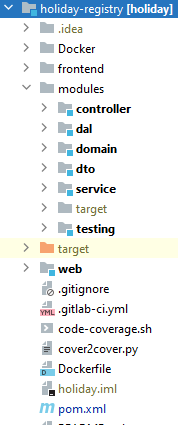
\includegraphics[scale=0.6]{images/mapstructure.png}
	\caption{Modularizált alkalmazás mappastruktúrája}
	\label{fig:mapstructure}
\end{figure}

A már részletesen ismertetett Többszintű alkalmazás felépítését tükrözi \aref{fig:mapstructure}. ábra. 
Az itt látható felosztásban a gyökér könyvtáron belül található a web module aminek jelenesetünkben csak konfigurációs szerepe van, mivel a spring-boot alkalmazások esetén a main függvényt tartalmazó osztálynak a csomaghierarchia legkülső csomagjában kell elhelyezkednie.

Amennyiben ez nem megfelelő helyen található az alkalmazásunk nem fogja látni a létrehozni kívánt komponenseket és a kontextust nem tudja felépíteni.

\paragraph{Frontend mappa}
Szintén leolvasható \aref{fig:mapstructure}. ábráról, hogy a jelen esetben struktúra részét képezi a megjelenítési réteghez szükséges applikációt tartalmazó mappa is. Mivel jelenleg nem microservice architektúrát alkalmazunk ez a megoldás is elfogadható, de gyakorlatban nem ajánlott és igen ritka.

\paragraph{Testing}
Ez egy úgynevezett rétegeken átívelő modul, aminek minden rétegben szerepe van, ebben a megvalósításban a modul nem tartalmaz kódot, csupán konfigurációt és a maven jacoco nevezetű teszt riport generáló kiegészítője által létrehozott fájlokat. Ezeket a fejlesztés során a tesztlefedettség méréséhez használjuk, képes vizualizációi segítségével megmutatni egy html oldalon, melyik osztályban milyen szintű a lefedettség, és azt is milyen hiányosságaink vannak tesztek terén.

\Section{Összetett objektum előállítása JSON formátumból Lombok használatával}

A szoftverfejlesztés egyik alapelve az, hogy ne ismételd önmagad, ami a redundanciából eredő hibalehetőségek és fejlesztési komplikációk csökkentése érdekében lett egy kitűzött cél. Az elv ellenére mégis rengeteg egyszerű kódsort ismételünk újra az Objektum Orientált fejlesztés során.

\subsection{Az ismétlődő programrészletek}

Minden általános java objektum létrehozásakor létrehozunk az osztály mezőihez:
\begin{itemize}
	\item legalább egy konstruktort,
	\item beállító és lekérdező függvényeket,
	\item titkosító valamint egyenlőség vizsgáló függvényeket,
	\item és a könnyebb hibakeresés érdekében, még egy kiíró függvényt is.
\end{itemize}

Ezek az implementációk legtöbbször annyira elemiek, hogy minden fejlesztőkörnyezet, automatikusan képes generálni a hozzájuk tartozó implementációt. Ez a sokszor több száz sornyi kódrészlet rengeteg tárhelyet jelent valamint tesztelés szempontjából ezek az osztályok többnyire rontják a lefedettséget. Mivel ezeknek a függvényeknek a tesztelése a nyelv működésére irányulna, így a saját alkalmazásunkban felesleges ezekre tesztesetet implementálni.

\subsection{A Lombok működése}
A felvázolt probléma megoldására született a Project Lombok\cite{lombok} könyvtár aminek a segítségével egyszerű annotációk használatával használhatjuk ezeket a kódrészleteket anélkül, hogy implementálnánk azokat a saját programunkban

\paragraph{@Data} használatával a mezők definiálása után rögtön használhatóvá válnak a már említett redundánsnak mondható kódok.
\begin{java}
	@Data
	public class UserEntity {
		private Long userId;
		private String email;
		private String password;
		private UserEntityRole role;
	}
	
\end{java}

\subsection{Megváltoztathatatlan objektumok Lombokban}
Objektum orientált programozásban gyakran használunk objektumokat adatok továbbítására, adattovábbítás esetén fontos, hogy gondosodjuk az objektum állapotáról. Amennyiben az változtatható a programozás, abban az esetben megnövekszik a hibalehetőségek száma.
\vskip 0.2in
Ahhoz, hogy ne lehessen bármikor megváltoztatni egy objektum mezőjének az állapotát, úgy kell megírni a hozzá tartozó függvényeket, hogy a mezőértékek csak és kizárólag a referencia létrehozásakor legyenek beállíthatóak.

A megoldás egy része igen egyszerű nem, hozunk létre olyan függvényeket ami példányosítást követően módosítani tudja az állapotot, tehát a beállító vagy más néven set függvényeket nem implementáljuk.

Ezáltal, viszont konstruktor argumentumokon keresztül lehet csak példányosítani, és ha esetleg adott esetben az egyik paraméter nem létezik ott, a példányosításkor null értéket kell átadnunk. Továbbá a paraméter sorrend is gondot okozhat ezért ez egy körülményes megoldás.

\paragraph{Építő minta} segítségével pontosan láthatjuk melyik mezőt definiáljuk és melyiket nem, ebben a megoldásban egy privát konstruktoron keresztül példányosítjuk az osztályunkat aminek a belső builder azaz epítő osztályán keresztül állítunk be.

\vskip 0.2in
Ez ismét a korábban említett problémakörhöz vezet, ezért a Lombok könyvtár erre is nyújt megoldást a \textbf{@Value} valamint a \textbf{@Builder} elölések használatával. 

Amíg az előbbi a megváltoztathatatlan osztály feltételeit teremti meg addig az utóbbi segítségével egy könnyen használható építő mintát megvalósító belső osztályt kapunk.

\subsection{JSON felépítésű String generálása Jacksonnal}

A Jackson könyvtár egy olyan megvalósítást kínál ami segítségével könnyedén alakíthatjuk át összetett java objektumainkat egy egyszerű JSON formátumú String értékké. 

Ennek a könyvtárnak a segítségével Belső modulban létező Holidayhistory.java osztályban található összetett objektum könnyedén átalakítható egy egyszerű String típussá és bármikor elvégezhető az átalakítás visszafelé is. 

A következő osztály struktúrából:
\begin{java}
public class HolidayHistory {	
	Long id;
	PersonDetails person;
	List<YearHistory> yearHistories;
}

public class YearHistory {
	int year;
	BigDecimal fixHolidaysForTheYear;
	List<EventRelatedHoliday> eventRelatedHolidays;
	List<HolidayEvent> holidayEvents;
}

public class EventRelatedHoliday {
	EventRelatedHolidayType holidayType;
	int days;
	LocalDate eventDate;
	LocalDate expiration;
}

public class HolidayEvent {
	String description;
	LocalDate startDate;
	LocalDate endDate;
	Boolean dadHoliday;
}
\end{java}

Az itt látható JSON értéket generálja ami már könnyedén menthető az adatbázisunkban.
\begin{java}
[
{
	"year": 2020,
	"fixHolidaysForTheYear": 10,
	"eventRelatedHolidays": [
	{
		"holidayType": "dad",
		"days": 0,
		"eventDate": "2021-03-30",
		"expiration": null
	},
	{
		"holidayType": "dad",
		"days": 0,
		"eventDate": "2021-03-30",
		"expiration": "2021-04-10"
	}
	],
	"holidayEvent": [
	{
		"description": "desc",
		"startDate": "2020-03-04",
		"endDate": "2020-05-20",
		"dadHoliday": null
	}
	]
},
{
	"year": 2021,
	"fixHolidaysForTheYear": 10,
	"eventRelatedHolidays": [
	{
		"holidayType": "dad",
		"days": 0,
		"eventDate": "2021-03-30",
		"expiration": null
	},
	{
		"holidayType": "dad",
		"days": 0,
		"eventDate": "2021-03-30",
		"expiration": "2021-04-10"
	}
	],
	"holidayEvent": null
}
]
\end{java}

A Jackson elap beállítás esetén a JSON létrehozásához a lekérdező függvényeket használja, így egyértelmű, hogy a JSON formátumból a beállító függvények segítségével állít elő objektumot.

Ahhoz, hogy a lombok és Jackson könyvtárak megfelelően működjenek együtt Megváltoztathatatlan objektumok létrehozása esetén az építő függvény további beállításaira valamint új annotációk használatára van szükségünk.

Minden érintett osztályt a következő alakra kell hozni.
\begin{java}
@Value
@Builder(builderClassName = "YearHistoryBuilder", 
access = AccessLevel.PUBLIC)
@JsonDeserialize(builder = 
YearHistory.YearHistoryBuilder.class)
@AllArgsConstructor(access = AccessLevel.PRIVATE)
public class YearHistory {
	
	@JsonProperty("year")
	int year;
	@JsonProperty("fixHolidaysForTheYear")
	BigDecimal fixHolidaysForTheYear;
	@JsonProperty("eventRelatedHolidays")
	List<EventRelatedHoliday> eventRelatedHolidays;
	@JsonProperty("holidayEvent")
	List<HolidayEvent> holidayEvents;
	
	@JsonPOJOBuilder(withPrefix = "")
	public static class YearHistoryBuilder {}
}
\end{java}  

Az itt látható alakban a Jackson könyvtár már képes azonosítani az átalakításhoz szükséges Lombok által biztosított függvényeket.

\Section{Automatizált Cron munkamenetek Springben}

Az automatizálás kulcsfontosságú szerepet játszik az alkalmazás piaci rést betöltő lehetőségeiben, ezért kifejezetten fontos, hogy a beállított időzített processzek fond nélkül végrehajtódjanak.

\paragraph{Java timer} segítségével képesek vagyunk másodpercben definiálni egy időzítőt ami az első indítástól számítva minden alkalommal folyamatosan számol és az időzítő lejártakor elindíthatunk egy feladatot vagy komplex feladat sort is.

Sajnos ez a megoldás nem megfelelő számunkra hiszen az időzítő minden újrainduláskor lefutna valamint akár kiszámíthatatlan viselkedést is generálhat.

\subsection{A keretrendszer nyújtotta előnyök}
A Spring keretrendszerben sok megbízható és könnyen alkalmazható megoldás található már létező problémákra, ezek közé tartozik az automatizált függvényhívások is.
\vskip 0.2in
A megoldás során a keretrendszer egy Cron munkamenetet, hoz létre az általunk konfigurált futási feltételeknek megfelelően, ez esetben nem az applikáció belső számlálója felel a függvényhívás elindításáért. A munkamenet a szerver számítógépen jön létre és minden alkalommal meghívja azt a függvényt amelyiken definiáltuk amennyiben az aktuális dátum és idő egyezik az általunk konfigurálttal.

\subsection{Cron munkamenet implementálása Spring-boot-ban}

A spring-boot applikáció indító függősége automatikusan tartalmazza a számunkra szükséges könyvtárakat, viszont az eléréséhez és használatához meg kell jelölnünk a megfelelő osztályokat és függvényeket.

\begin{java}
	@SpringBootApplication
	@EnableScheduling
	public class HolidayApplication {...}
\end{java}

Engedélyezést követően az applikáció kontextusában bármelyik nyilvános függvényünk megjelölésével létrehozhatunk egy új munkamenetet.

\begin{java}
@Scheduled(cron = "1 0 0 * * ?")
public void schedule() {
	unusedHolidaysService.addPenalty();
	childBornHolidaysService.validate();
}
\end{java}

Léteznek előre definiált beállítások z automatizált futtatáshoz, de ahogy a kódrészlet is mutatja bármikor konfigurálhatunk saját feltételeket, a cron leírónyelv segítségével.

A nyelvben hat karaktert kell megadnunk amik jelentését \aref{tab:Cron leírónyelv} táblázat tartalmazza:

\begin{table}[h]
	\centering
	\caption{Cron leírónyelv értékei.}
	\label{tab:Cron leírónyelv}
\begin{tabular}{|c|c|c|c|}
	\hline
	Érték & Kötelező & Megengedett értékek & Speciális karakterek \\
	\hline
	Másodperc & Igen & 0-59 & , - * / \\
	\hline
	Perc & Igen & 0-59 & , - * / \\
	\hline
	Óra & Igen & 0-23 & , - * / \\
	\hline
	Hónap napja & Igen & 1-31 & , - * ? / L W C \\
	\hline
	Hónap & Igen & 0-11 vagy JAN-DEC & , - * / \\
	\hline
	Hét napja & Igen & 1-7 vagy SUN-SAT & , - * ? / L C \# \\
	\hline
	Év & Nem & üres vagy 1970-2099 & , - * / \\
	\hline
\end{tabular}
\end{table}

\Section{Automatizált szabadság számolás tört év esetén, Nemzeti ünnepek tárolása}

Az automatizálás folyamatát és a törvényben leírt szabályoknak megfelelő számítást ismerve könnyedén megvalósíthatunk egy összetett hívási láncot amely végén az éves vagy akaár a részarányos szabadnapok számolása megtörténik.
A kihívást jelentő probléma az egyenletben egyedül, az aktuális éveben hátralévő munkanapok száma jelenti, ehhez ugyanis minden számolás esetén tudnunk kell a tárgy évben mennyi olyan munkanap létezik amely az aktuális nemzet számára munkaszüneti napnak minősül.
\vskip 0.2in
Habár a szóban forgó dátumok többsége állandó és az ezekre vonatkozó megoldás kézenfekvő, mozgó ünnepek esetén nem tárolhatunk állandó értéket. 

\subsection{Külső API hívása}
Kisebb kereséssel rengeteg számunkra hasznos szolgáltatást találhatunk ahol, egy bizonyos URL összeállításával és a mögötte található végpont meghívásával minden szükséges információhoz hozzájuthatunk.

A legegyszerűbb verzió visszatérési értéke teljes mértékben tökéletes lenne számunkra hiszen tartalmazza azt a számot amit felhasználva csak be kell helyettesítenünk az egyenletünkbe.

Több lehetőség van amelynél az adott év vagy nap adatainak megadása esetén visszakapjuk, hogy az munkanap vagy sem.
\vskip0.2in
A legnagyobb probléma viszont ezekkel az elérhető alkalmazásokkal, hogy az ingyenes hozzáférésük szigorúan korlátozva van, havi vagy éves előfizetésük pedig jelen esetben nem összeegyeztethető ár érték arányban az igényeinkkel.

\subsection{Mozgó ünnepek számolása}

A külső API hívások nélkül a legkézenfekvőbb megoldása az automatizálásnak, hogy saját magunk számoljuk ki az adott dátumok értékeit, ehhez könnyedén találhatunk számolásokat. 

Ezekről a számolásokról viszont elmondhatjuk, hogy nem adnak valós értéket, különböző tényezők miatt hónapokat tévedhetnek, így kis utánajárással kideríthetjük, hogy a jelenleg kiszámolt mozgó ünnepek dátumai egyrészt számoláson másrészt megegyezésen alapulnak.

Kimondhatjuk tehát, hogy saját számolások elvégzése, jelen esetben nem megvalósítható.

\subsection{Félautomata megoldás}

A végleges megoldás egy részben manuális karbantartást igénylő implementáció, melynek során az állandó dátummal rendelkező dátumok első beállítást követően újra számolódnak, a nem változó dátum jelölés esetén viszont az adminisztrátorra bízzuk a konfigurációt.

\Section{Folyamatos Integráció beállítása Gitlabon}

A már említett CI/CD folyamatok beállítása nagy segítséget tud nyújtani és a fejlesztést is meggyorsíthatja, a kódbázis felépítése és a tesztek futtatása idő és erőforrás igényes lehet a saját számítógépünkön, így ezt a munkát delegálva időt nyerhetünk. 

A gitlab verziókezelő szolgáltatás lehetőséget nyújt saját Folyamatos integrációs csővezeték definiálásra amiben, az építés, a tesztek futtatása és a generált adatok alapján a tesztlefedettséget mérő munkameneteket könnyedén definiálhatjuk.

\subsection{.gitlab-ci.yml konfiguráció}

A gitlab szolgáltatásának részét képezi az alap szintű integrációs folyamatok létrehozása, ezek indulása automatikus. Nekünk csupán egy konfigurációs .yml kiterjesztésű fileban kell definiálnunk az általunk futtatni kívánt folyamatokat és az azokhoz tartozó esetleges környezeti változókat, vagy parancsokat.

A stages érték megadása után definiálnunk kell a munkamenetek nevét és sorrendjét.
 \begin{python}
 	stages:
 	  - build
 	  - test
 	  - coverage
 \end{python} 

Ezután konfiguráljuk a munkamenet, úgy hogy hivatkozunk a nevére majd megadjuk, hogy milyen docker image környezetben fusson az adott folyamat.

\begin{python}
	build:
	  stage: build
	  image: maven:3.6.3-jdk-11
\end{python}

Legvégül a script érték alatt  felsoroljuk milyen parancsokat hajtson végre a docker imagen belül. 
\begin{python}
	script:
	  - mvn $MAVEN_CLI_OPTS compile
	  
\end{python}

\subsection{További felhasználható funkció}
Ez a gyors konfiguráció nem csak a fejlesztést gyorsíthatja fel de akár Folyamatos szállítást is definiálhatunk vele, egy olyan munkamenet segítségével ami a felépített alkalmazásunk futtatható .war vagy .jar kiterjesztésű futtatható elemeit becsomagolja egy docker konténerbe, ssh kapcsolatot létesít egy általunk definiált IP címmel és ott a megadott helyre kitelepíti az alkalmazásunkat.

Ezzel elérhetjük, hogy a felhasználó a nap végére akár több hibajavítás eredményét vagy akár pár hetente egy új funkció használatát is élvezhesse. 